\chapter{Proof of Concept}
\label{ch:poc}
In dit hoofdstuk lichten we de opzet en implementatie van de proof of concept applicatie toe. 
Deze applicatie is ontwikkeld als \textbf{Progressive Web App (PWA)} en stelt gebruikers in staat om videofragmenten te analyseren en met elkaar te vergelijken op basis van de houding en bewegingen die erin worden gedetecteerd. 
Daarnaast bespreken we waarom we hebben gekozen voor het gebruik van \textbf{TensorFlow.js} om het pose-detectiemodel in de browseromgeving te implementeren, en hoe dit model technisch geïntegreerd werd in de applicatie.

\section{Progressive Web App (PWA)}
De proof of concept is ontwikkeld als een \textbf{Progressive Web App}, een moderne webtoepassing die zich gedraagt als een native app op zowel mobiele toestellen als desktops. 
PWAs combineren de voordelen van een website en een mobiele app:
\begin{itemize}
    \item \textbf{Toegankelijkheid}: gebruikers kunnen de applicatie rechtstreeks via de browser gebruiken, zonder installatie via een app store.
    \item \textbf{Offline functionaliteit}: met caching en service workers kan de applicatie ook zonder internetverbinding functioneren.
    \item \textbf{Platformonafhankelijkheid}: één codebase werkt op verschillende besturingssystemen en apparaten.
    \item \textbf{Veiligheid en updates}: PWAs draaien in een veilige sandbox-omgeving en zijn eenvoudig te updaten via de webserver.
\end{itemize}

Dankzij deze eigenschappen sluit een PWA perfect aan bij het doel van dit onderzoek, namelijk het ontwikkelen van een gebruiksvriendelijke en technisch haalbare mobiele applicatie die personal trainers en fitnesscoaches in staat stelt om nauwkeurige bewegingsfeedback te geven aan hun cliënten.

\section{TensorFlow.js}
Voor de implementatie van MoveNet-model in de browser is gebruikgemaakt van \textbf{TensorFlow.js}, een krachtige machine learning-bibliotheek die toelaat om modellen direct in JavaScript uit te voeren. 
Dit sluit perfect aan bij een PWA, die volledig in JavaScript of TypeScript wordt ontwikkeld.

\section{Analyse en visualisatie}
De applicatie laat gebruikers toe om een referentievideo en een eigen videofragment op te laden. 
De referentievideo is een opname van een correcte uitvoering van een oefening, terwijl de gebruikersvideo de eigen uitvoering van de gebruiker bevat (zie Figuur~\ref{fig:upload_page}).

\begin{figure}[H]
  \centering
  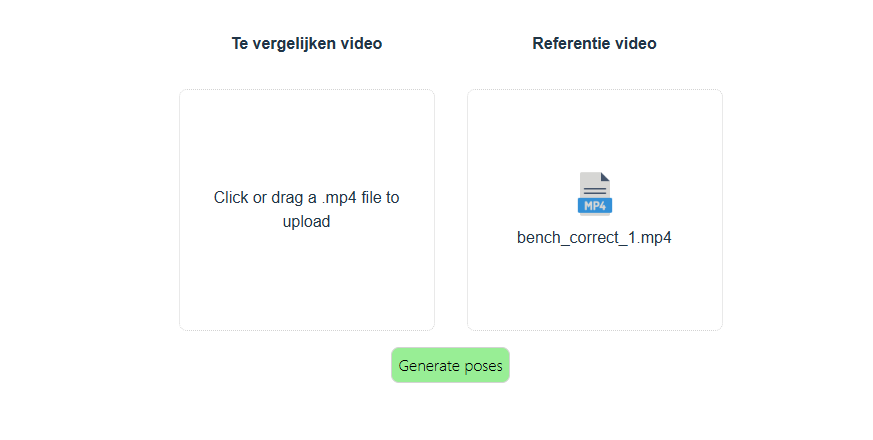
\includegraphics[width=0.8\textwidth]{upload-page.png}
  \caption[Upload page]{\label{fig:upload_page}Uploadpagina van de PWA}
\end{figure}

Beide video’s worden afzonderlijk geanalyseerd, waarbij de poses per frame worden berekend. 
Vervolgens worden de hoeken van de gewrichten bepaald, waarmee een vergelijking gemaakt kan worden tussen beide video’s met behulp van het uiteengezette algoritme uit het vorige hoofdstuk.

Tijdens het afspelen worden de referentievideo en de vergelijkingsvideo gelijktijdig afgespeeld. Op de referentievideo worden de hoeken visueel weergegeven:
\begin{itemize}
    \item Elke verbinding tussen gewrichten krijgt een kleur afhankelijk van de mate van afwijking ten opzichte van de referentie:
    \begin{itemize}
        \item \textbf{Groen}: kleine of geen afwijking.
        \item \textbf{Rood}: significante afwijking.
    \end{itemize}
    \item Deze kleurcodering stelt de gebruiker in staat om snel visueel te zien waar en wanneer tijdens de oefening verbeterpunten zich voordoen.
\end{itemize}

\begin{figure}[h]
  \centering
  \begin{minipage}{0.45\textwidth}
      \centering
      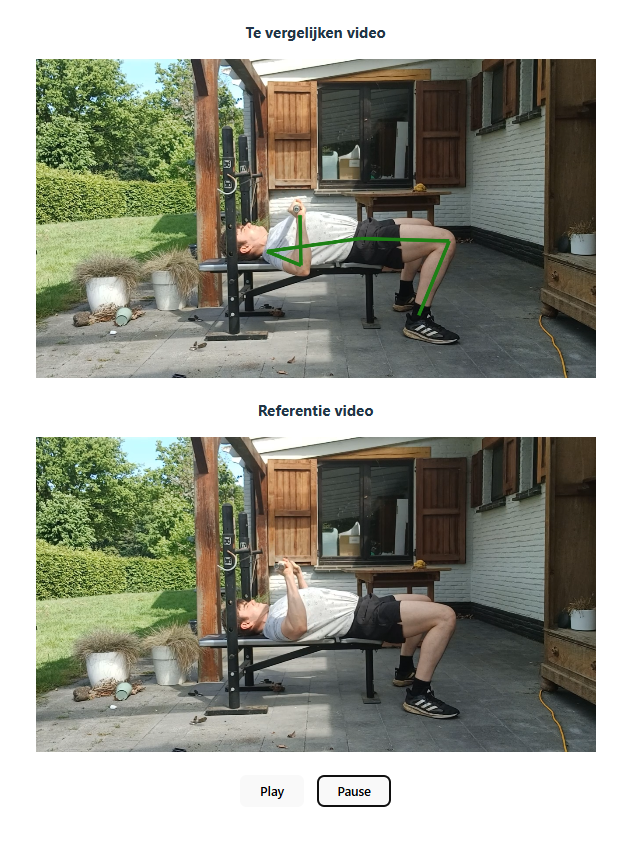
\includegraphics[width=\linewidth]{green-comparison.png}
      \caption[Weinig afwijking]{\label{fig:green_comparison}Uitvoeringen met weinig afwijkingen}
  \end{minipage}
  \hfill % Voegt wat ruimte toe tussen de afbeeldingen
  \begin{minipage}{0.45\textwidth}
      \centering
      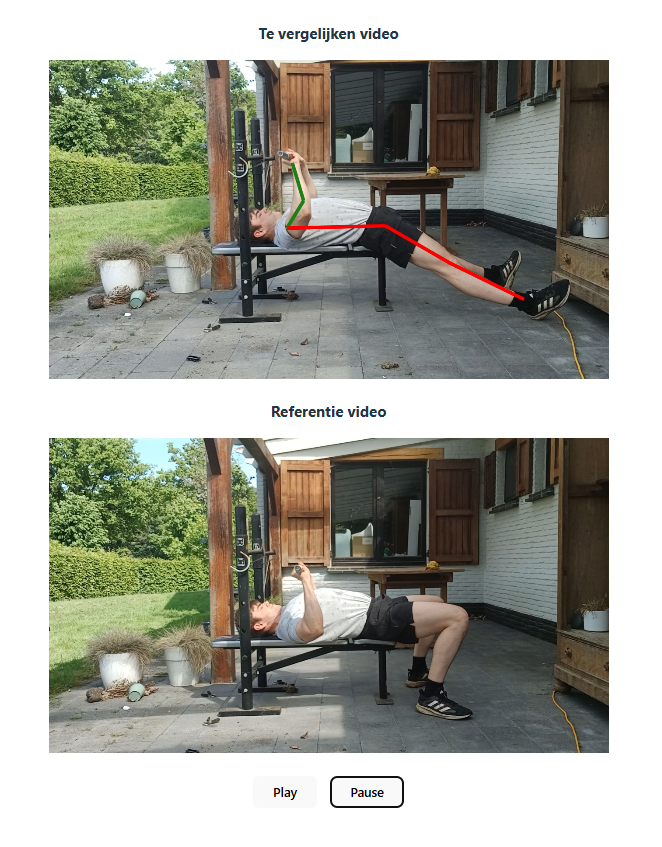
\includegraphics[width=\linewidth]{red-comparison.png}
      \caption[significante afwijking]{\label{fig:red_comparison}Uitvoeringen met significante afwijkingen}
  \end{minipage}
\end{figure}   
